\documentclass[12pt]{article}

\usepackage[utf8]{inputenc}
\usepackage[english]{babel}
\usepackage{amssymb}
\usepackage{amsfonts}
\usepackage{amsmath}
\usepackage{graphicx}
\usepackage[margin=1in]{geometry}
\usepackage[hidelinks]{hyperref}
\usepackage{float}
\usepackage[danish]{varioref}
\usepackage{multirow}
\usepackage{hhline}
\usepackage{inconsolata}
\usepackage{etoolbox}
\usepackage[usenames,dvipsnames]{xcolor}
\usepackage{tikz}
\usetikzlibrary{positioning,shapes, shadows, arrows}
\usepackage{listings}

%%%%%%%%%%%%%%%%%%%%%%%%%
%   subsubsubsection    %

\usepackage{titlesec}
\titleclass{\subsubsubsection}{straight}[\subsection]

\newcounter{subsubsubsection}[subsubsection]
\renewcommand\thesubsubsubsection{\thesubsubsection.\arabic{subsubsubsection}}

\titleformat{\subsubsubsection}
  {\normalfont\normalsize\bfseries}{\thesubsubsubsection}{1em}{}
\titlespacing*{\subsubsubsection}
{0pt}{3.25ex plus 1ex minus .2ex}{1.5ex plus .2ex}

\makeatletter
\def\toclevel@subsubsubsection{4}
\def\l@subsubsubsection{\@dottedtocline{4}{7em}{4em}}
\makeatother

\setcounter{secnumdepth}{4}
\setcounter{tocdepth}{4}

%                       %
%%%%%%%%%%%%%%%%%%%%%%%%%

\setlength\parindent{0pt}
\usepackage[parfill]{parskip}

\definecolor{dark-blue}{HTML}{000080}
\definecolor{dark-green}{HTML}{008000}
\definecolor{pale-purple}{HTML}{94558D}
\definecolor{dark-purple}{HTML}{0000AA}
\definecolor{regular-purple}{HTML}{660099}
\definecolor{magenta}{HTML}{B200B2}
\definecolor{light-gray}{HTML}{FAFAFA}
\definecolor{dark-gray}{HTML}{2D2D2D}
\definecolor{comment}{HTML}{808080}
\definecolor{digit}{HTML}{0000FF}

\newcommand*{\FormatDigit}[1]{\textcolor{digit}{#1}}

\lstset{
	language=Ruby,
	prebreak=\raisebox{0ex}[0ex][0ex]{\ensuremath{\color{red}\space\hookleftarrow}},
	basicstyle=\footnotesize\ttfamily,
	%
	literate=%
    	{0}{{\FormatDigit{0}}}{1}%
        {1}{{\FormatDigit{1}}}{1}%
        {2}{{\FormatDigit{2}}}{1}%
        {3}{{\FormatDigit{3}}}{1}%
        {4}{{\FormatDigit{4}}}{1}%
        {5}{{\FormatDigit{5}}}{1}%
        {6}{{\FormatDigit{6}}}{1}%
        {7}{{\FormatDigit{7}}}{1}%
        {8}{{\FormatDigit{8}}}{1}%
        {9}{{\FormatDigit{9}}}{1}%
        {.0}{{\FormatDigit{.0}}}{2}% Following is to ensure that only periods
        {.1}{{\FormatDigit{.1}}}{2}% followed by a digit are changed.
        {.2}{{\FormatDigit{.2}}}{2}%
        {.3}{{\FormatDigit{.3}}}{2}%
        {.4}{{\FormatDigit{.4}}}{2}%
        {.5}{{\FormatDigit{.5}}}{2}%
        {.6}{{\FormatDigit{.6}}}{2}%
        {.7}{{\FormatDigit{.7}}}{2}%
        {.8}{{\FormatDigit{.8}}}{2}%
        {.9}{{\FormatDigit{.9}}}{2}%
        %{,}{{\FormatDigit{,}}{1}% depends if you want the "," in color
        {\ }{{ }}{1}% handle the space
		{æ}{{\ae}}1
        {ø}{{\o}}1
        {å}{{\aa}}1
        {Æ}{{\AE}}1	
        {Ø}{{\O}}1
        {Å}{{\AA}}1
        {~}{{$\scriptstyle{\sim}$}}1, % handle tilde ~
	%
	%emph={},
	otherkeywords={},
	keywords=[2]{self},
	keywords=[3]{__init__},
	keywords=[4]{object},
	keywords=[5]{encoding, flags},
	keywords=[6]{reduce,list,enumerate,len,map,range,sorted,None,super},
	%
	keywordstyle=\bfseries\color{dark-blue},
	keywordstyle={[2]\color{pale-purple}},
	keywordstyle={[3]\color{magenta}},
	keywordstyle={[4]\color{dark-blue}},
	keywordstyle={[5]\color{regular-purple}},
	keywordstyle={[6]\color{dark-purple}},
    commentstyle=\itshape\color{comment},
    identifierstyle=\color{black},
	stringstyle=\bfseries\color{dark-green},
	%emphstyle=\color{dark-purple},
	%
	numbers=left, % where to put the line-numbers
	numberstyle=\ttfamily\color{dark-gray},
	numbersep=5pt, % how far the line-numbers are from the code
	stepnumber=1,
	showstringspaces=false,
	backgroundcolor=\color{light-gray},
	tabsize=4,
	captionpos=b, % sets the caption-position to bottom
	breaklines=true % sets automatic line breaking
}

\linespread{1.3}

\begin{document}

\begin{titlepage}
    \vspace*{\fill}
    \begin{center}
      {\Huge Midtvejsrapport Bachelorproject}\\[0.7cm]
      {\Large Regular Expression Matching In Genomic Data}\\[0.4cm]
      {\large Rasmus Haarslev - nkh877}\\
      {\large Troels Thomsen - qvw203}\\[0.4cm]
      {Supervisors: Rasmus Fonseca}\\
      {\small 23. Februar 2015}\\[0.3cm] 
      {\small Department of Computer Science}\\
      {\small University of Copenhagen}
    \end{center}
    \vspace*{\fill}
\end{titlepage}	

\clearpage
\pagenumbering{gobble}
\thispagestyle{empty}

\newpage

\tableofcontents
\newpage

\pagenumbering{arabic}

\section{Problem definition}

We wish to determine the possibility of converting sequence analysis patterns used for scan-for-matches\cite{scan-for-matches}, into regular expressions\cite{crash-course-regex} and test their efficiency against the KMC\cite{kmc-website} engine.

Specifically we wish to solve the following problems:

\begin{itemize}
	\item Is it possible to programatically convert patterns used by the scan-for-matches program into regular expressions for the KMC engine? If not all patterns used by scan-for-matches then which ones?
	\item Is it possible to achieve speeds matching or exceeding scan-for-matches with the generated regular expressions and the KMC engine?
	\item Can we find weak extensions to regular expressions, which would enable us to support more or all scan-for-matches patterns?
\end{itemize}

\newpage

\section{Introduction}

Scan for matches is a program developed by Ross Overbeek, David Joerg and Morgan Price, which is able to locate complex DNA patterns. These patterns are written in its own format, which from now on will be referred to as patscan patterns.\cite{scan-for-matches}

The most notable of the patscan format's features, is the possibility to search for mismatches, insertions and deletions in a given sequence. The sequence \texttt{AGTCT} can be extended to \texttt{AGTCT[1,1,1]} in order to match upto one mismatch, upto one insertion, upto one deletion or any combination of thereof.

This means that a sequence of length $n$ with a single mismatch will yield $n^1+1$ possible matches. \texttt{AGTCT[1,0,0]} will for instance match any of the following, where \_ represents a mismatch.

\texttt{AGTCT, \_GTCT, A\_TCT, AG\_CT, AGT\_T, AGTC\_}

If we extrapolate into $m$ mismatches, $d$ deletions and $i$ insertions, we quickly find ourselves with approximately  $n^{m^{d^{i}}}+1$ possible matches, since all of our mismatches can be combined with all of our deletions, which in turn can be combined with all of our insertions.

Combining this match combination notation with the ability to store sequences in variables and matching them further down the pattern, makes the patscan format a powerful tool in regards to searching DNA. \\
A pattern as simple as \texttt{p1=AGTCC p1 10...50 p1[2,0,1]} describes a complex relationship, which cannot easily be discovered through conventional search methods.

\newpage

\section{What is regular expressions}

\newpage

\section{Translation of scan-for-matches patterns into regular expressions}

\subsection{Grammar}

The patscan grammar can roughly be summarized as the following: \\

\begin{tabular}{ p{5cm} | l | l }
	\textbf{Token type} & \textbf{Regular expression} & \textbf{Example} \\
    \hline
    Sequence & 
  	{\begin{lstlisting}[numbers=none, backgroundcolor=\color{white}]
^[a-z]+$ 
	\end{lstlisting}} & 
    {\begin{lstlisting}[numbers=none, backgroundcolor=\color{white}]
AGTCT
	\end{lstlisting}} \\
    \hline
    Sequence with mismatches, insertions and deletions & 
	{\begin{lstlisting}[numbers=none, backgroundcolor=\color{white}]
^[a-z]+\[[0-9]+,[0-9]+,[0-9]+\]$ 
	\end{lstlisting}} &
    {\begin{lstlisting}[numbers=none, backgroundcolor=\color{white}]
AGTCT[1,0,0]
	\end{lstlisting}} \\
    \hline
    Range & 
	{\begin{lstlisting}[numbers=none, backgroundcolor=\color{white}]
^[0-9]+\.{3}[0-9]+$
	\end{lstlisting}} & 
	{\begin{lstlisting}[numbers=none, backgroundcolor=\color{white}]
2...4
	\end{lstlisting}} \\
    \hline
    Variable assignment & 
    {\begin{lstlisting}[numbers=none, backgroundcolor=\color{white}]
^[^=]+=[^=]+$
	\end{lstlisting}} & 
    {\begin{lstlisting}[numbers=none, backgroundcolor=\color{white}]
p1=AGTCT
	\end{lstlisting}} \\
    \hline
    Variable usage &
	{\begin{lstlisting}[numbers=none, backgroundcolor=\color{white}]
^~?[\^{}=]+$ 
	\end{lstlisting}} &
    {\begin{lstlisting}[numbers=none, backgroundcolor=\color{white}]
~p1
	\end{lstlisting}} \\
\end{tabular}

\subsection{Mismatches, Insertions and Deletions}

The sub-patterns can have the following form, which allows for mismatches, insertions and deletions in the sub-pattern. 

\begin{equation}
	x_1 \ldots x_n[m, i, d] \ \ \{ x_1 \ldots x_n \in A \ | \ m, i, d \in \mathbb{N}_0 \}
\end{equation} 

This notation allows for 0 or the given number of mismatches, insertions or deletions, or all possible combinations in between. This means we for example can have $m$ mismatches and $i$ insertions, but not necessarily $d$ deletions.

Translating these sub-patterns is not a simple task. This kind of notation doesn't exist in regular expressions. Hence, the only way to represent them, is by constructing every possible combination of the sequence, matching the pat\_scan notation. To give an example, the pattern \texttt{AAG[1,0,0]} will translate into

\begin{eqnarray}
	((AAG)|([\ \hat{}A]AG)|(A[\ \hat{}A]G)|(AA[\ \hat{}G]))
\end{eqnarray}

Starting with mismatches only, writing a general algorithm to translate this example is fairly simple, but becomes increasingly more difficult, as the sequence becomes longer, and especially when the number of allowed mismatches are increased.

We had different approaches to this problem, as we developed our translator. Our first approach was loops. Implementing the translation using only loops to iterate over every combination seemed like the easiest and simplest way to tackle the problem.

\subsubsection{Loops}

Implementing a single mismatch, using loops, were simple. A single loop, choosing a different character for the mismatch in each iteration (as well as the sequence without mismatches).

For two mismatches, it was still fairly simple, we had to use a nested loop this time, that each corresponded to one of the mismatches. We just had to also include all the combinations from the previous iterations, that only had a single mismatch.

This approach seem to rely on implementing an algorithm for each number of mismatches, and then concatenating them. This is a problem, because there can be an arbitrary number of mismatches. It is very impractical to implement enough, and simply impossible to implement them all. Combining this with insertions and deletions, and we have a real headache on hand.

\subsubsection{Recursion}

The second approach was recursion. With recursion, it was much easier to implement a general model of translation. The way implemented this, was to look at each character one at a time, and look at all the possibilities of what that character could be.

This way, we could construct a recursion tree, that is capable of generating all possible combinations, no matter how many mismatches is allowed.

For just mismatches, the recursion tree would build two new branches per iteration. The first iteration of \texttt{AGCTC[2,0,0]} would build the branches

\begin{eqnarray}
	Left\ branch &=& A\{GCTC[2,0,0]\} \\
	right\ branch &=&\ \hat{}A\{GCTC[1,0,0]\}
\end{eqnarray}

Here, the left branch will continue recursively with \texttt{GCTC[2,0,0]}, and the right branch will do the same, but with only one mismatch available. On the deepest recursion level of each branch, we will have a string, with a unique combination of mismatches.

Simply speaking, for mismatches, each character can be $N \in \{n, \hat{}n\}$

Adding deletions, this set $N$ will become one larger, and so will the number of recursion branches created in each iteration. Insertions on top of this, besides other problems, that insertions create, increases this number of recursions further.

The recursion does not stop before every combination is found. This is a problem, because if the sequence is large enough (This can happen already at a length of 20, if not earlier, depending on the number of mismatches, insertions, and deletions), the computer will run out of memory, if the program doesn't stop it before that happens.

\subsubsection{Divide and Conquer}

\subsection{Variable assignments}



\section{Application flow chart}

\subsection{Lexer}
\begin{figure}[H]
	\begin{center}
		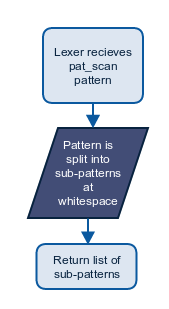
\includegraphics[scale=1]{lexer.png}
	\end{center}
	\caption{Flow chart of our lexer}
\end{figure}

Pat\_scan sub-patterns are always separated by whitespace characters. Because of this, and because of the fact, that the grammar is very simple, we can simply split the pat\_scan pattern at all whitespace, and we're left with a list of each sub-pattern.

\subsection{Parser}
\begin{figure}[H]
	\begin{center}
		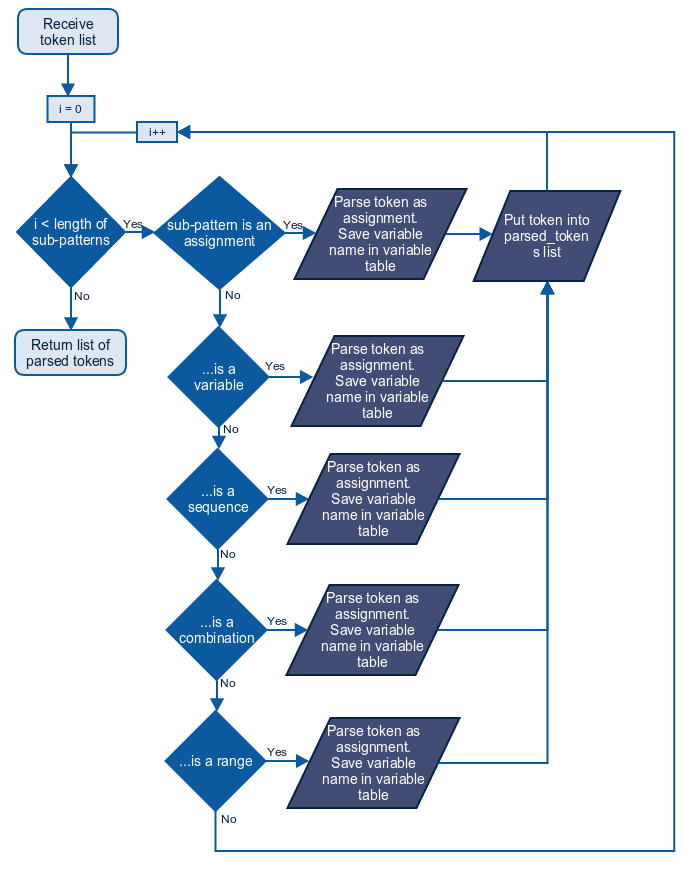
\includegraphics[scale=0.65]{parser.png}
	\end{center}	
	\caption{Flow chart of our parser}
\end{figure}

The parser takes each token from the received token list, and checks them against our grammar, and depending on which type of sub-pattern it is, it will be parsed as such. Each parsed sub-pattern will then be put into a list, which will be returned in the end.

The way, which tokens are parsed, is they are being put into a Token object, which takes a pattern type and a match object. The pattern type is so that the translator can recognize which type of sub-pattern the token is. The match object is the object returned when our grammar matched the token successfully. 

This way, we assign names to specific parts of the sub-pattern, so they're easily accessible for the translator. This could for instance be the number of mismatches in a pattern such as \texttt{AGTCA[2,0,0]}

\newpage

\bibliographystyle{plain}
%\nocite{*}
\bibliography{litterature}

\end{document}
